\documentclass{article}

\usepackage{graphicx}
\usepackage{tikz}
\usepackage{tikzsymbols}
\usetikzlibrary{calc,patterns,shapes.geometric}
\pagestyle{empty}
\usepackage[margin=0pt]{geometry}
\geometry{papersize={14in,12in}}

\def\centerarc[#1](#2)(#3:#4:#5){\draw[#1] ($(#2)+({#5*cos(#3)},{#5*sin(#3)})$) arc (#3:#4:#5);}

\begin{document}
	\begin{figure}
		\centering
		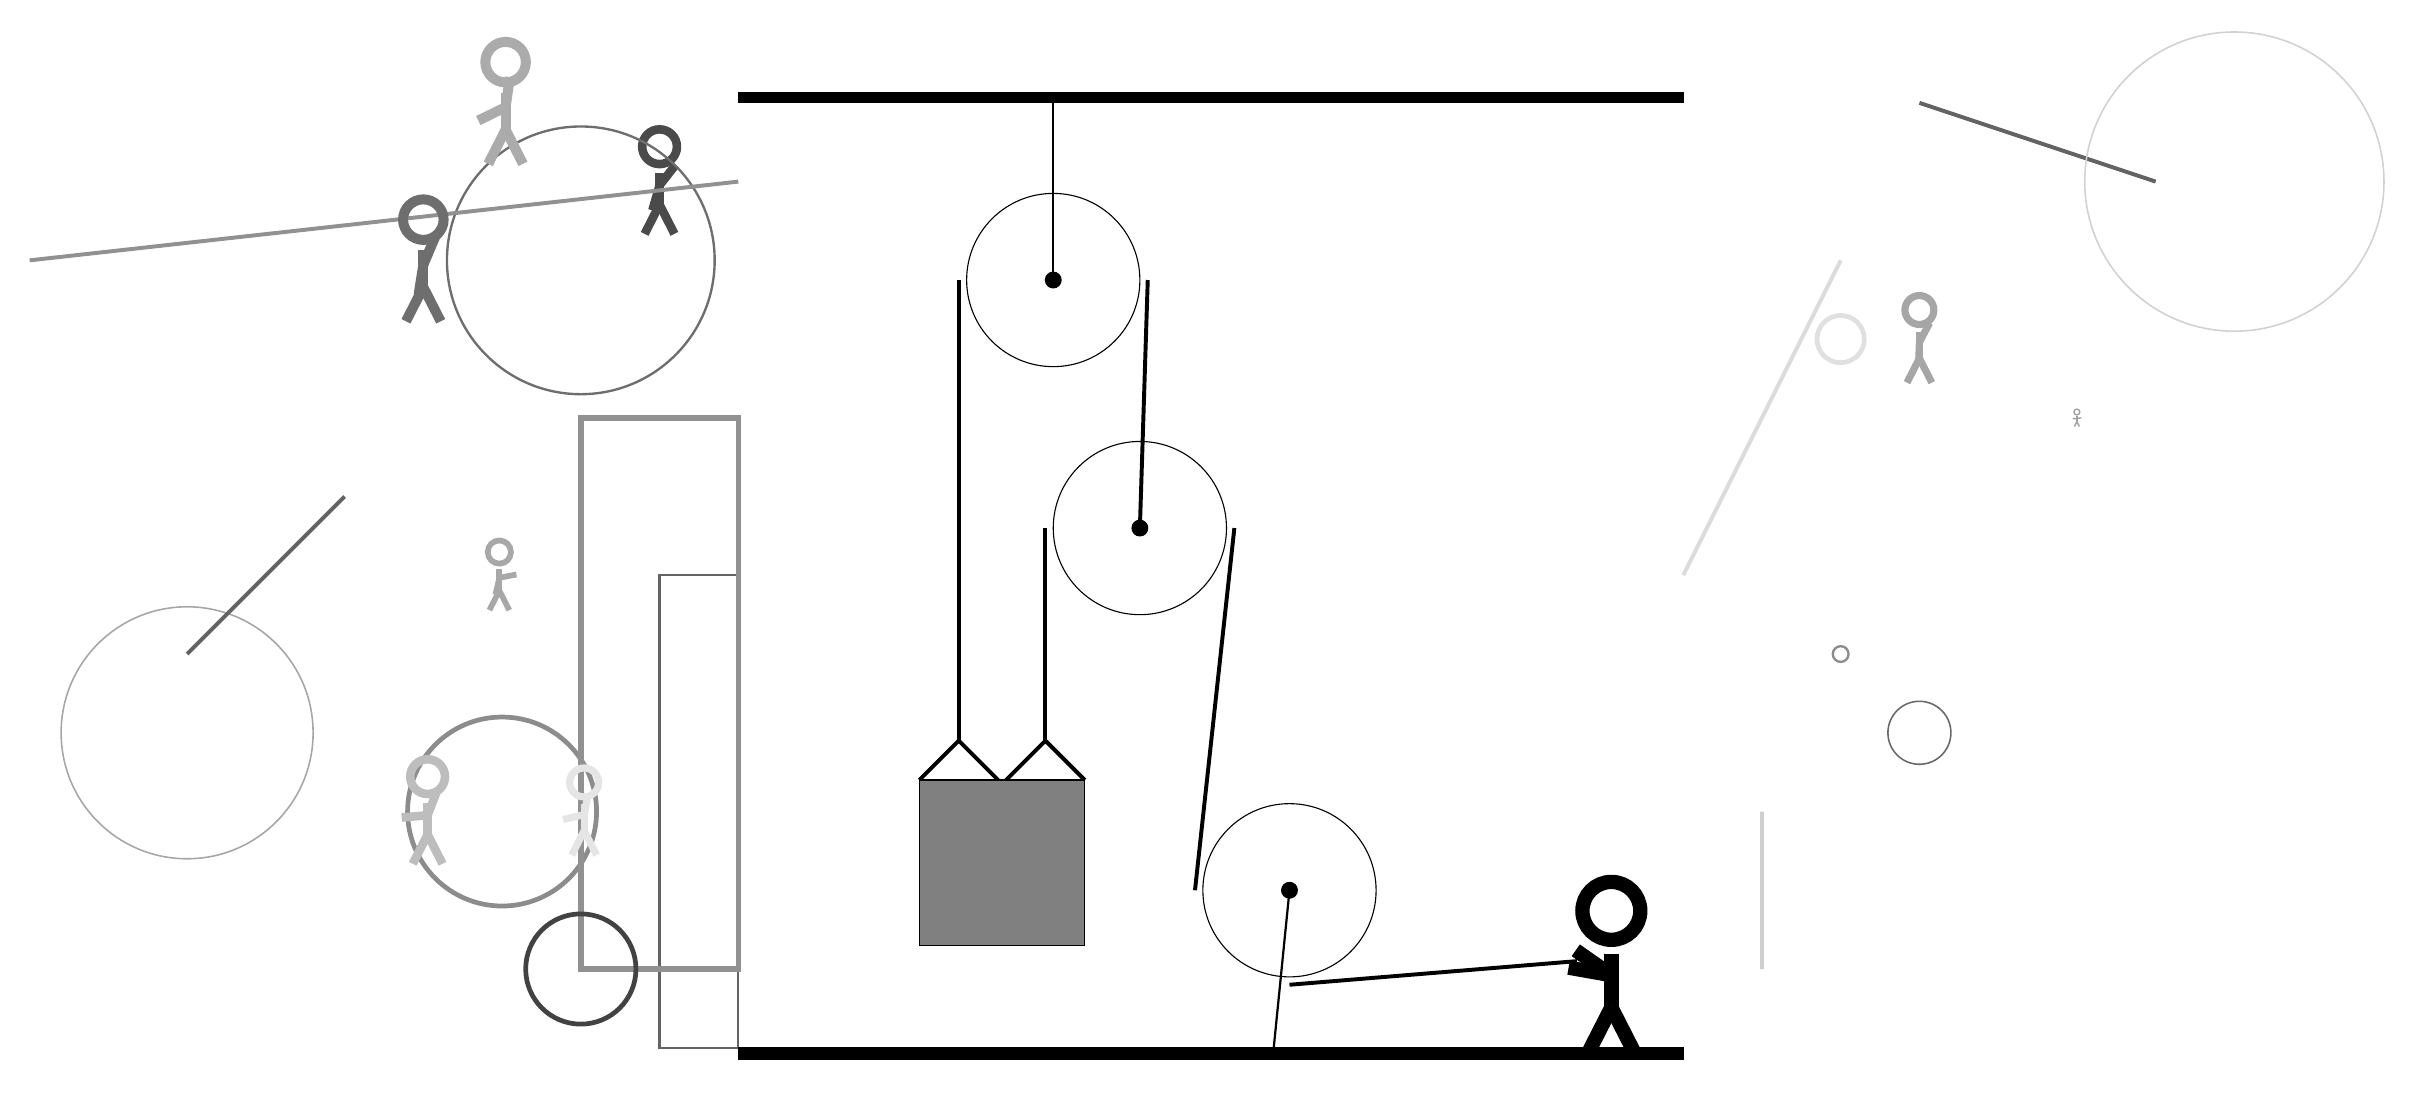
\begin{tikzpicture}
			%%%%% START %%%%%
			
			\draw[fill=black] (-2, 9) rectangle (10, 9.125);
			
			\draw (2, 6.75) circle (1.1);
			\draw[fill=black] (2, 6.75) circle (0.1);
			\draw[thick] (2, 6.75) -- (2, 9);
			
			\draw (3.1, 3.6) circle (1.1);
			\draw[fill=black] (3.1, 3.6) circle (0.1);
			
			\draw (5, -1) circle (1.1);
			\draw[fill=black] (5, -1) circle (0.1);
			\draw[thick] (5, -1) -- (4.8, -3);
			
			\draw[line width = 0.5mm]  (0.3, 0.4) -- (0.8, 0.9) -- (1.3, 0.4);
			\draw[line width = 0.5mm]  (1.4, 0.4) -- (1.9, 0.9) -- (2.4, 0.4);
			\draw[fill=black!50] (0.3, 0.4) rectangle (2.4, -1.7);
			
			\draw[line width = 0.5mm] (0.8, 6.75) -- (0.8, 0.9);
			\centerarc[line width = 0.5mm](2, 6.75)(0:180:1.2000000000000002);
			\draw[line width = 0.5mm] (3.2, 6.75) -- (3.1, 3.6);
			\draw[line width = 0.5mm] (1.9, 3.6) -- (1.9, 0.9);
			\centerarc[line width = 0.5mm](3.1, 3.6)(0:180:1.2000000000000002);
			\draw[line width = 0.5mm] (4.3, 3.6) -- (3.8, -1);
			\centerarc[line width = 0.5mm](5, -1)(180:270:1.2000000000000002);
			\draw[line width = 0.5mm] (5, -2.2) -- (8.65, -1.9);
			
			\node at (9, -2) {\Strichmaxerl[10][-35][170]};
			
			\draw [line width=0.3mm, color=black!45](12, 2) circle (0.1);
			
			\node[line width=0.5mm, color=black!34] at (-5, 3) {\Strichmaxerl[4][77][11]};
			\node[line width=0.2mm, color=black!71] at (-3, 8) {\Strichmaxerl[6][74][52]};
			\draw[line width=0.3mm, color=black!61] (-2, -3) rectangle (-3, 3);
			
			\node[line width=0.3mm, color=black!37] at (15, 5) {\Strichmaxerl[1][3][8]};
			
			\draw [line width=0.3mm, color=black!57](-4, 7) circle (1.7);
			\draw [line width=0.6mm, color=black!45](-5, 0) circle (1.2);
			
			\draw[line width=0.5mm, color=black!61](13, 9) -- (16, 8);
			\draw[line width=0.7mm, color=black!43] (-4, -2) rectangle (-2, 5);
			
			\node[line width=0.2mm, color=black!10] at (-4, 0) {\Strichmaxerl[5][13][79]};
			
			\node[line width=0.2mm, color=black!33] at (-5, 9) {\Strichmaxerl[7][26][82]};
			\draw [line width=0.6mm, color=black!12](12, 6) circle (0.3);
			\draw [line width=0.6mm, color=black!74](-4, -2) circle (0.7);
			
			\draw[line width=0.5mm, color=black!43](-2, 8) -- (-11, 7);
			\node[line width=0.6mm, color=black!57] at (-6, 7) {\Strichmaxerl[7][81][67]};
			\draw [line width=0.2mm, color=black!18](17, 8) circle (1.9);
			
			\draw[line width=0.5mm, color=black!14](10, 3) -- (12, 7);
			\node[line width=0.5mm, color=black!35] at (13, 6) {\Strichmaxerl[5][88][62]};
			\draw [line width=0.2mm, color=black!59](13, 1) circle (0.4);
			\node[line width=0.6mm, color=black!26] at (-6, 0) {\Strichmaxerl[6][5][69]};
			\draw[line width=0.5mm, color=black!19] (11, -2) rectangle (11, 0);
			\draw [line width=0.2mm, color=black!35](-9, 1) circle (1.6);
			\draw[line width=0.5mm, color=black!61](-7, 4) -- (-9, 2);
			
			\draw[fill=black] (-2, -3) rectangle (10, -3.15);
			
			%%%%% END %%%%%
		\end{tikzpicture}
	\end{figure}	
\end{document}